
\documentclass{beamer}
\usetheme{Madrid}

\title{Building a GNU/Hurd Cluster}
\author{Brent Baccala}
\institute{\tt cosine@freesoft.org}
\date{January 17, 2018}

\setbeamertemplate{footline}{}
\beamertemplatenavigationsymbolsempty

\usepackage{xcolor}
\usepackage{comment}
\usepackage{graphicx}

\usepackage{tabularx}

\usepackage{xstring}

\usepackage{tikz}
\usetikzlibrary{positioning, fit, backgrounds, arrows, patterns}

\begin{document}

\begin{frame}
\titlepage
\begin{block}{Abstract}
The GNU Hurd is a UNIX-like operating system based on Mach, an
operating system kernel developed at Carnegie Mellon University and
designed to support multi-node clusters, which have become ubiquitous
in high performance computing.  This talk will highlight current
trends in cluster computing, outline the design of Mach and Hurd, and
summarize the speaker's work to realize Hurd's potential as a
POSIX-compatible operating system that can leverage the power of an
entire cluster.
\end{block}
\end{frame}

\newcommand\topfh[7]{
#1 & #2 & #3 & #4 & #6 & #7 \\
& \multicolumn{4}{l}{\hskip 1cm #5} \\
\\
}

\begin{frame}
\frametitle{Top 10 positions of the TOP500 (November 2017)}
{\tiny
\begin{tabularx}{\textwidth}{lllllll}
\bf Rank
& \bf Name
& \bf Processor
& \bf Vendor
& \bf Cores
& \bf Operating system
\\
\\
\topfh{1}
{Sunway TaihuLight}
{SW26010}
{NRCPC}
{National Supercomputing Center in Wuxi, CHN}
{10,649,600}
{Linux (Raise)}

\topfh{2}
{Tianhe-2}
{Xeon E5–2692, Xeon Phi 31S1P}
{NUDT}
{National Supercomputing Center in Guangzhou, CHN}
{3,120,000}
{Linux (Kylin)}

\topfh{3}
{Piz Daint}
{Xeon E5-2690v3, Nvidia Tesla P100}
{Cray}
{Swiss National Supercomputing Centre, SWI}
{361,760}
{Linux (CLE)}

\topfh{4}
{Gyoukou}
{Xeon D-1571, PEZY-SC2}
{ExaScaler}
{Japan Agency for Marine-Earth Science and Technology, JAP}
{19,860,000}
{Linux (CentOS)}

\topfh{5}
{Titan}
{Opteron 6274, Nvidia Tesla K20X}
{Cray}
{Oak Ridge National Laboratory, USA}
{560,640}
{Linux (CLE, SLES based)}

\topfh{6}
{Sequoia}
{IBM A2}
{IBM}
{Lawrence Livermore National Laboratory, USA}
{1,572,864}
{Linux (RHEL and CNK)}

\topfh{7}
{Trinity}
{Xeon E5–2698v3, Xeon Phi}
{Cray}
{Los Alamos National Laboratory, USA}
{979,968}
{Linux (CLE)}

\topfh{8}
{Cori}
{Xeon Phi 7250}
{Cray}
{National Energy Research Scientific Computing Center, USA}
{622,336}
{Linux (CLE)}

\topfh{9}
{Oakforest-PACS}
{Xeon Phi 7250}
{Fujitsu}
{Kashiwa, Joint Center for Advanced High Performance Computing, JPN}
{556,104}
{Linux}

\topfh{10}
{K computer}
{SPARC64 VIIIfx}
{Fujitsu}
{Riken, Advanced Institute for Computational Science (AICS), JPN}
{705,024}
{Linux}

\end{tabularx}
Source: {\tt https://www.top500.org/}
}
\end{frame}

\begin{frame}
\frametitle{Cisco 5108 Blade Server Chassis with eight B200 M2s}
\includegraphics[width=\textwidth]{ourcisco.jpg}
\end{frame}

\begin{frame}
\frametitle{Processor families in TOP500}
\includegraphics[width=\textwidth]{Processor_families_in_TOP500_supercomputers.png}
\end{frame}

\begin{frame}
\frametitle{Techniques to exploit parallelism}
\begin{itemize}
\item Instruction level parallelism
\begin{itemize}
\item Superscalar vector operations
\item Speculative execution
\item Co-processors
\end{itemize}
\item Thread level parallelism
\begin{itemize}
\item Shared memory
\item Caching
\item Synchronization
\end{itemize}
\item Node level parallelism
\begin{itemize}
\item No shared memory
\item High speed LAN
\item Clusters
\end{itemize}
\end{itemize}
\end{frame}

\begin{frame}[fragile]
\frametitle{Adding 512 64-bit integers - conventional x86-64 instrs}
\begin{semiverbatim}
\tiny
int a[512];
int b[512];
int c[512];

int main () \{
  for (int i=0; i<512; i++) \{
    c[i] = a[i] + b[i];
  \}
\}


baccala@ideapad-S510p:~\$ gcc -O2 -fno-align-loops -o ex1 ex1.c


00000000004003e0 <main>:
4003e0:31 c0                xor    %eax,%eax
4003e2:8b 90 60 18 60 00    mov    0x601860(%rax),%edx
4003e8:03 90 60 10 60 00    add    0x601060(%rax),%edx
4003ee:48 83 c0 04          add    $0x4,%rax
4003f2:89 90 5c 20 60 00    mov    %edx,0x60205c(%rax)
4003f8:48 3d 00 08 00 00    cmp    $0x800,%rax
4003fe:75 e2                jne    4003e2 <main+0x2>
400400:31 c0                xor    %eax,%eax
400402:c3                   retq   

\end{semiverbatim}
\vskip 0pt plus 100fill
\end{frame}

\begin{frame}[fragile]
\frametitle{Adding 512 64-bit integers - SSE superscalar instructions}
\begin{semiverbatim}
\tiny
int a[512];
int b[512];
int c[512];

int main () \{
  for (int i=0; i<512; i++) \{
    c[i] = a[i] + b[i];
  \}
\}


baccala@ideapad-S510p:~$ gcc -O3 -fno-align-loops -o ex1 ex1.c


00000000004003e0 <main>:
4003e0:31 c0                         xor    %eax,%eax
4003e2:66 0f 6f 80 60 10 60 00       movdqa 0x601060(%rax),%xmm0
4003ea:48 83 c0 10                   add    $0x10,%rax
4003ee:66 0f fe 80 50 18 60 00       paddd  0x601850(%rax),%xmm0
4003f6:0f 29 80 50 20 60 00          movaps %xmm0,0x602050(%rax)
4003fd:48 3d 00 08 00 00             cmp    $0x800,%rax
400403:75 dd                         jne    4003e2 <main+0x2>
400405:31 c0                         xor    %eax,%eax
400407:c3                            retq   

\end{semiverbatim}
\vskip 0pt plus 100fill
\end{frame}

\begin{frame}[fragile]
\frametitle{Adding 512 64-bit integers - AVX2 superscalar instructions}
\begin{semiverbatim}
\tiny
int a[512] __attribute__((aligned(32)));
int b[512] __attribute__((aligned(32)));
int c[512] __attribute__((aligned(32)));

int main () \{
  for (int i=0; i<512; i++) \{
    c[i] = a[i] + b[i];
  \}
\}


baccala@ideapad-S510p:~$ gcc -march=native -O3 -o ex2 ex2.c


00000000004003e0 <main>:
4003e0:31 c0                         xor    %eax,%eax
4003e2:c5 fd 6f 80 60 10 60 00       vmovdqa 0x601060(%rax),%ymm0
4003ea:c5 fd fe 80 60 18 60 00       vpaddd 0x601860(%rax),%ymm0,%ymm0
4003f2:48 83 c0 20                   add    $0x20,%rax
4003f6:c5 fd 7f 80 40 20 60 00       vmovdqa %ymm0,0x602040(%rax)
4003fe:48 3d 00 08 00 00             cmp    $0x800,%rax
400404:75 dc                         jne    4003e2 <main+0x2>
400406:c5 f8 77                      vzeroupper 
400409:31 c0                         xor    %eax,%eax
40040b:c3                            retq   

\end{semiverbatim}
\vskip 0pt plus 100fill
\end{frame}

\begin{frame}[fragile]
\frametitle{Adding 512 64-bit integers - AVX512 superscalar instrs}
\begin{semiverbatim}
\tiny
int a[512] __attribute__((aligned(64)));
int b[512] __attribute__((aligned(64)));
int c[512] __attribute__((aligned(64)));

int main () \{
  for (int i=0; i<512; i++) \{
    c[i] = a[i] + b[i];
  \}
\}


baccala@ideapad-S510p:~$ gcc -mavx512vl -O3 -o ex3 ex3.c


00000000004003e0 <main>:
4003e0:31 c0                         xor    %eax,%eax
4003e2:62 f1 fd 48 6f 80 80 10 60 00 vmovdqa64 0x601080(%rax),%zmm0
4003ec:48 83 c0 40                   add    $0x40,%rax
4003f0:62 f1 7d 48 fe 80 40 18 60 00 vpaddd 0x601840(%rax),%zmm0,%zmm0
4003fa:62 f1 fd 48 7f 80 40 20 60 00 vmovdqa64 %zmm0,0x602040(%rax)
400404:48 3d 00 08 00 00             cmp    $0x800,%rax
40040a:75 d6                         jne    4003e2 <main+0x2>
40040c:31 c0                         xor    %eax,%eax
40040e:c3                            retq   

baccala@ideapad-S510p:~$ ./ex3
Illegal instruction (core dumped)
baccala@ideapad-S510p:~$ ./ex3

\end{semiverbatim}
\vskip 0pt plus 100fill
\end{frame}

\begin{frame}[fragile]
\frametitle{Pointer Aliasing}
\begin{semiverbatim}
\tiny
void operation (int * ap, int * bp, int * cp)
\{
  for (int i=0; i<16; i++) \{
    cp[i] = ap[i] + bp[i];
  \}
\}
\end{semiverbatim}
\pause
\begin{semiverbatim}
\tiny
int v[18] = \{1, 1\};

int main () \{
  operation(\&v[0], \&v[1], \&v[2]);

  for (int i=0; i<18; i++) \{
    printf("%d ", v[i]);
  \}
  printf("\\n");
\}
\end{semiverbatim}
What does this code do?
\pause
\begin{semiverbatim}
\tiny
baccala@blade6:~\$ ./ex4
1 1 2 3 5 8 13 21 34 55 89 144 233 377 610 987 1597 2584 
baccala@blade6:~\$
\end{semiverbatim}
\end{frame}


\begin{frame}[fragile]
\frametitle{Pointer Aliasing - The {\tt restrict} keyword}
\begin{semiverbatim}
\tiny
void operation (int * restrict a, int * restrict b, int * restrict c)
\{
  for (int i=0; i<16; i++) \{
    a[i] = b[i] + c[i];
  \}
\}


gcc -mavx512vl -O3 -c ex3.c

0000000000000000 <operation>:
   0:   62 f1 7e 48 6f 06       vmovdqu32 (%rsi),%zmm0
   6:   62 f1 7d 48 fe 02       vpaddd (%rdx),%zmm0,%zmm0
   c:   62 f1 7e 48 7f 07       vmovdqu32 %zmm0,(%rdi)
  12:   c3                      retq   

\end{semiverbatim}
\end{frame}

\begin{frame}
\frametitle{Intel Ivy Bridge Processor}
\includegraphics[width=\textwidth]{ivybridge.jpg}
\begin{center}
\huge
Notice the size of the graphics co-processor!
\end{center}
\end{frame}

\begin{frame}[fragile]
\frametitle{{\tt clDeviceQuery} on an Intel\textsuperscript{\textregistered} Core\texttrademark\ i5-4200U CPU}
\begin{semiverbatim}
\tiny
  CL_DEVICE_NAME:                       Intel(R) HD Graphics Haswell Ultrabook GT2 Mobile
  CL_DEVICE_VENDOR:                     Intel
  CL_DRIVER_VERSION:                    1.1.1
  CL_DEVICE_TYPE:                       CL_DEVICE_TYPE_GPU
  CL_DEVICE_MAX_COMPUTE_UNITS:          20
  CL_DEVICE_MAX_WORK_ITEM_DIMENSIONS:   3
  CL_DEVICE_MAX_WORK_ITEM_SIZES:        512 / 512 / 512 
  CL_DEVICE_MAX_WORK_GROUP_SIZE:        512
  CL_DEVICE_MAX_CLOCK_FREQUENCY:        1000 MHz
  CL_DEVICE_ADDRESS_BITS:               32
  CL_DEVICE_MAX_MEM_ALLOC_SIZE:         1024 MByte
  CL_DEVICE_GLOBAL_MEM_SIZE:            2048 MByte
  CL_DEVICE_ERROR_CORRECTION_SUPPORT:   no
  CL_DEVICE_LOCAL_MEM_TYPE:             global
  CL_DEVICE_LOCAL_MEM_SIZE:             64 KByte
  CL_DEVICE_MAX_CONSTANT_BUFFER_SIZE:   131072 KByte
  CL_DEVICE_QUEUE_PROPERTIES:           CL_QUEUE_PROFILING_ENABLE
  CL_DEVICE_IMAGE_SUPPORT:              1
  CL_DEVICE_MAX_READ_IMAGE_ARGS:        128
  CL_DEVICE_MAX_WRITE_IMAGE_ARGS:       8

  CL_DEVICE_IMAGE <dim>                 2D_MAX_WIDTH     8192
                                        2D_MAX_HEIGHT    8192
                                        3D_MAX_WIDTH     8192
                                        3D_MAX_HEIGHT    8192
                                        3D_MAX_DEPTH     2048

  CL_DEVICE_PREFERRED_VECTOR_WIDTH_<t>  CHAR 16, SHORT 8, INT 4, LONG 2, FLOAT 4, DOUBLE 0
\end{semiverbatim}
\end{frame}

\begin{frame}
\frametitle{Cluster Computing - History}
\begin{itemize}
\item Beowulf
\item Hadoop
\item Cluster Linux
\begin{itemize}
\item Kerrighed - Latest version is 3.0.0 which was released on 14 June 2010 and based on Linux kernel 2.6.30.
\item OpenSSI - last development release 2010; last stable release 2007
\end{itemize}
\end{itemize}
\end{frame}

\begin{comment}
\begin{frame}[fragile]
\begin{semiverbatim}
\tiny
import java.io.IOException;
import java.util.StringTokenizer;

import org.apache.hadoop.conf.Configuration;
import org.apache.hadoop.fs.Path;
import org.apache.hadoop.io.IntWritable;
import org.apache.hadoop.io.Text;
import org.apache.hadoop.mapreduce.Job;
import org.apache.hadoop.mapreduce.Mapper;
import org.apache.hadoop.mapreduce.Reducer;
import org.apache.hadoop.mapreduce.lib.input.FileInputFormat;
import org.apache.hadoop.mapreduce.lib.output.FileOutputFormat;

public class WordCount \{

  public static class TokenizerMapper
       extends Mapper<Object, Text, Text, IntWritable>\{

    private final static IntWritable one = new IntWritable(1);
    private Text word = new Text();

    public void map(Object key, Text value, Context context
                    ) throws IOException, InterruptedException \{
      StringTokenizer itr = new StringTokenizer(value.toString());
      while (itr.hasMoreTokens()) \{
        word.set(itr.nextToken());
        context.write(word, one);
      \}
    \}
  \}

  public static class IntSumReducer
       extends Reducer<Text,IntWritable,Text,IntWritable> \{
    private IntWritable result = new IntWritable();

    public void reduce(Text key, Iterable<IntWritable> values,
                       Context context
                       ) throws IOException, InterruptedException \{
      int sum = 0;
      for (IntWritable val : values) \{
        sum += val.get();
      \}
      result.set(sum);
      context.write(key, result);
    \}
  \}

  public static void main(String[] args) throws Exception \{
    Configuration conf = new Configuration();
    Job job = Job.getInstance(conf, ``word count'');
    job.setJarByClass(WordCount.class);
    job.setMapperClass(TokenizerMapper.class);
    job.setCombinerClass(IntSumReducer.class);
    job.setReducerClass(IntSumReducer.class);
    job.setOutputKeyClass(Text.class);
    job.setOutputValueClass(IntWritable.class);
    FileInputFormat.addInputPath(job, new Path(args[0]));
    FileOutputFormat.setOutputPath(job, new Path(args[1]));
    System.exit(job.waitForCompletion(true) ? 0 : 1);
  \}
\}
\end{semiverbatim}
\end{frame}
\end{comment}

\begin{frame}[fragile]
\frametitle{Hadoop MapReduce Tutorial - WordCount}
\begin{semiverbatim}
\tiny public class WordCount \{

  public static class TokenizerMapper
       extends Mapper<Object, Text, Text, IntWritable>\{

    private final static IntWritable one = new IntWritable(1);
    private Text word = new Text();

    public void map(Object key, Text value, Context context)
                     throws IOException, InterruptedException \{
      StringTokenizer itr = new StringTokenizer(value.toString());
      while (itr.hasMoreTokens()) \{
        word.set(itr.nextToken());
        context.write(word, one);
      \}
    \}
  \}

  public static class IntSumReducer
       extends Reducer<Text,IntWritable,Text,IntWritable> \{
    private IntWritable result = new IntWritable();

    public void reduce(Text key, Iterable<IntWritable> values, Context context)
                        throws IOException, InterruptedException \{
      int sum = 0;
      for (IntWritable val : values) \{
        sum += val.get();
      \}
      result.set(sum);
      context.write(key, result);
    \}
  \}
\}
\end{semiverbatim}
\end{frame}

\begin{frame}[fragile]
\frametitle{Single System Image}
\begin{definition}
A single system image (SSI) cluster is a cluster of machines that appears to be one single system.

\hfill Wikipedia
\end{definition}
\begin{center}
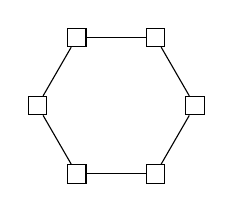
\begin{tikzpicture}
\node (a) [draw] at (0:1) {};
\node (b) [draw] at (60:1) {} edge (a);
\node (c) [draw] at (120:1) {} edge (b);
\node (d) [draw] at (180:1) {} edge (c);
\node (e) [draw] at (240:1) {} edge (d);
\node (f) [draw] at (300:1) {} edge (e) edge (a);
\end{tikzpicture}
\end{center}
\begin{semiverbatim}
\$ nproc
96
\$ free -h
              total        used        free
Mem:           768G         45G        723G
Swap:            0B          0B          0B

\end{semiverbatim}
\end{frame}

\begin{frame}
\frametitle{Single System Image}

\begin{itemize}
\item Key Features
\begin{itemize}
\item Cluster-wide login
\item Single Process Space
\item Process Migration
\item Single Root Filesystem
\item Redundant Filesystem
\item Single I/O Space - block devices
\item Single IPC Space
standard Linux inter-process communication mechanisms, shared memory, semaphores, SYSV message queues, pipes and Unix domain sockets.
\item Cluster-wide IP Addresses
\end{itemize}
\item Advantages
\begin{itemize}
\item familiar programming and management tools
\item ease of leveraging additional computing power
\end{itemize}
\item Disadvantages
\begin{itemize}
\item less fault isolation
\item node failure more difficult
\end{itemize}
\end{itemize}
\end{frame}

\begin{frame}
\frametitle{Single System Image - History}
\begin{itemize}
\item VMS
\item SCALEMP
\item Cluster Linux
\end{itemize}
\end{frame}

\begin{frame}
\frametitle{GNU Hurd}
\begin{itemize}
\item History
\item Microkernels in general
\item CMU Mach
\end{itemize}
\end{frame}

\begin{frame}
\frametitle{CMU Mach}
\begin{itemize}
\item Tasks / Threads
\item Interprocess Communication
\item Memory Management
\end{itemize}
\end{frame}

% tikz commands to draw task boxes to illustrate Mach IPC concepts

\tikzstyle{task} = [draw, fill=blue!20, rounded corners]

\tikzstyle{kernel} = [draw, fill=blue!20, rounded corners, minimum width=30em, minimum height=8em]

\tikzstyle{message} = [draw, fill=red!20, text width=5em, text depth=3em, text centered,
  minimum width=5em, minimum height=2em, rounded corners]

% \task - takes four arguments
% 1. name of task (used to refer to it from tikz; maybe printed as a label as well)
% 2. location of task box's center point
% 3. "r" or "l", indicating if a set of tick marks representing
%    ports should drawn on the left or right side of the task box
%    "u" to label the task "Task" instead of labeling it with its name
%    "b" to make a "big" node (I wish I knew how to size the tick marks automatically)
% 4. contents of the task box - other nodes
%
% The tick marks will be named "#1 Port #" for future reference

\newcommand\task[4]{
\matrix (#1) [task, inner xsep=0] at (#2) { \node {\IfSubStr{#3}{u}{Task}{#1}}; \\ #4

% print port tick marks in fill color if they are disabled, in order to make
% them expand out the dimensions of the task box yet remain invisible

\foreach \i in {-7,...,7}
{
\IfSubStr{#3}{l}{
  \draw[xshift=-5em, ultra thick] (0,0.2 * \i)  coordinate (#1 Port \i) -- (0.2,0.2 * \i);
}{
  \draw[xshift=-5em, ultra thick, color=blue!20] (0,0.2 * \i) -- (0.2,0.2 * \i);
}
\IfSubStr{#3}{r}{
  \draw[xshift=5em, ultra thick] (-0.2,0.2 * \i) -- (0,0.2 * \i) coordinate (#1 Port \i);
}{
  \draw[xshift=5em, ultra thick, color=blue!20] (-0.2,0.2 * \i) -- (0,0.2 * \i);
}
}

\\};
}

\newcommand\bigtask[4]{
\matrix (#1) [task, inner xsep=0] at (#2) { \node {\IfSubStr{#3}{u}{Task}{#1}}; \\ #4

% print port tick marks in fill color if they are disabled, in order to make
% them expand out the dimensions of the task box yet remain invisible

\foreach \i in {-20,...,7}
{
\IfSubStr{#3}{l}{
  \draw[xshift=-5em, ultra thick] (0,0.2 * \i)  coordinate (#1 Port \i) -- (0.2,0.2 * \i);
}{
  \draw[xshift=-5em, ultra thick, color=blue!20] (0,0.2 * \i) -- (0.2,0.2 * \i);
}
\IfSubStr{#3}{r}{
  \draw[xshift=5em, ultra thick] (-0.2,0.2 * \i) -- (0,0.2 * \i) coordinate (#1 Port \i);
}{
  \draw[xshift=5em, ultra thick, color=blue!20] (-0.2,0.2 * \i) -- (0,0.2 * \i);
}
}

\\};
}

% draw a box with vertical lines to represent a message queue
% arg 1 is the name of a port to position it to the left of
% arg 2 is name to be given the box

\newcommand\queue[2]{
\filldraw (#1) +(-3.1,0) node[rectangle, name=#2, minimum width=1.8cm, minimum height=1cm, draw, pattern=vertical lines] {};
}

\begin{frame}
\frametitle{Ports - Mach's Interprocess Communication (IPC)}

\begin{center}

\begin{tikzpicture}[transform canvas={scale=0.4, yshift=12em, xshift=-15em}]

\task{Task 1 left}{0,0}{ru}{}
\task{Task 2 left}{0,-11 em}{ru}{}
\task{Task 3 left}{0,-22 em}{ru}{}
\task{Task 4 left}{0,-33 em}{ru}{}
\task{Task 1 right}{30 em,0}{lu}{}
\task{Task 2 right}{30 em,-11 em}{lu}{}
\task{Task 3 right}{30 em,-22 em}{lu}{}
\task{Task 4 right}{30 em,-33 em}{lu}{}

\queue{Task 1 right Port 5}{queue 1}
\queue{Task 2 right Port -5}{queue 2a}
\queue{Task 2 right Port 5}{queue 2b}
\queue{Task 3 right Port 0}{queue 3}
\queue{Task 4 right Port 0}{queue 4}

\draw [color=violet, thick, -triangle 90] (Task 1 left Port 5) -- (queue 1.west);
\draw [color=violet, thick, -triangle 90] (queue 1.east) -- (Task 1 right Port 5);
\draw [color=violet, thick] (Task 2 left Port 0) -- +(1,0) |- (queue 1.west);
\draw [color=violet, thick, -triangle 90] (Task 2 left Port -3) -- +(1,0) |- (queue 4.west);

\draw [color=violet, thick, -triangle 90] (Task 2 left Port 5) -- (queue 2b.west);
\draw [color=violet, thick, triangle 90-] (Task 2 left Port -5) -- (queue 2a.west);
\draw [color=violet, thick, -triangle 90] (queue 2b.east) -- (Task 2 right Port 5);
\draw [color=violet, thick, triangle 90-] (queue 2a.east) -- (Task 2 right Port -5);

\draw [color=violet, thick, -triangle 90] (Task 3 left Port 0) -- (queue 3.west);
\draw [color=violet, thick, -triangle 90] (queue 3.east) -- (Task 3 right Port 0);

\draw [color=violet, thick, -triangle 90] (Task 3 right Port 0) ++(-1,0) |- ++(-4,1) -- ++(0,-1);

\draw [color=violet, thick, -triangle 90] (queue 4.east) -- (Task 4 right Port 0);

\draw [color=violet, thick, -triangle 90] (Task 4 left Port 3) -- +(2,0) |- +(6,5.5) |- (queue 2a.east);


\end{tikzpicture}
\end{center}

\end{frame}

\begin{frame}
\frametitle{Mach IPC}

\begin{center}

\begin{tikzpicture}

\task{Task 1}{0,0}{r}{
\node (message1) [message] {Message 1};
}
\task{Task 2}{15 em,0}{l}{
\node (message2) [message] at (1 em, 1 em) {Message 1};
\node (message2a) [message] at (1.9 em, -1 em) {Message 2};
}
\task{Task 3}{0,-11 em}{r}{
\node (message3) [message] {Message 2};
}


\draw [color=violet, thick, ->] (node cs:name=message1,angle=20) -- +(.3,0) |- (Task 1 Port 5) node [midway, anchor=south, color=black] {27} -- (Task 2 Port 5)
    -- +(.5,0) node [at end, anchor=south, color=black] {52} |- (node cs:name=message2, angle=160);

\draw [color=violet, thick, ->] (node cs:name=message3,angle=0) -- +(.3,0) |- (Task 3 Port 0) node [midway, anchor=south, color=black] {18} -- +(1,0) |- (Task 2 Port 5)
    -- +(.5,0) |- (node cs:name=message2a, angle=160);

\end{tikzpicture}
\end{center}

\end{frame}

\begin{frame}
\frametitle{Transfering a Send Right}
\begin{center}
\begin{tikzpicture}[node distance = .5cm]

\bigtask{Task 1}{0,0}{r}{
% print two sendright nodes, one to fill the message1 box to the correct size,
% and another one to actually draw it, since message1 will overwrite the
% first sendright
\only<2->{
\node (sendright) [draw, fill=orange] {Send 41};
\node (message1) [fit=(sendright), message] {Message 1};
\node (sendright) [draw, fill=orange] {Send 41};
}

\only<4->{\node (message3) at (0, -7em) [message] {Message 2};}
}

\bigtask{Task 2}{15 em,0}{l}{
\only<3->{
\node (sendright2) [draw, fill=orange] {Send 9};
\node (message2) [fit=(sendright2), message] {Message 1};
\node (sendright2) [draw, fill=orange] {Send 9};
}

\only<4->{\node (message4) at (0, -7em) [message] {Message 2};}
}

\only<2->{\node (port 41) [left of=Task 1 Port -10, anchor=south] {41};}

\only<2->{\draw [thick, color=red, dotted, ->] (node cs:name=sendright, angle=-20) -- (port 41);}

\node [left of=Task 1 Port 5, anchor=south] {27};
\node [right of=Task 2 Port 5, anchor=south] {52};
\only<1,2>{\draw [thick, -triangle 90] (Task 1 Port 5) -- (Task 2 Port 5);}

\only<3->{
\draw [color=violet, thick, -triangle 90] (node cs:name=message1,angle=20) -- +(.3,0) |- (Task 1 Port 5) -- (Task 2 Port 5)
    -- +(.5,0) |- (node cs:name=message2, angle=160);
}

\only<3->{\node [right of=Task 2 Port -10, anchor=south] {9};}

\only<3>{\draw [thick, triangle 90-] (Task 1 Port -10) -- (Task 2 Port -10);}

\only<4->{
\draw [color=violet, thick, triangle 90-] (node cs:name=message3,angle=20) -- +(.3,0) |- (Task 1 Port -10) -- (Task 2 Port -10)
    -- +(.5,0) |- (node cs:name=message4, angle=160);
}

\end{tikzpicture}
\end{center}
\end{frame}

\begin{frame}
\frametitle{Transfering a Receive Right}
\begin{center}
\begin{tikzpicture}[node distance = .5cm]

\bigtask{Task 1}{0,0}{r}{
% print two sendright nodes, one to fill the message1 box to the correct size,
% and another one to actually draw it, since message1 will overwrite the
% first sendright
\only<2->{
\node (sendright) [draw, fill=green] {Recv 41};
\node (message1) [fit=(sendright), message] {Message 1};
\node (sendright) [draw, fill=green] {Recv 41};
}

\only<4->{\node (message3) at (0, -7em) [message] {Message 2};}
}

\bigtask{Task 2}{15 em,0}{l}{
\only<3->{
\node (sendright2) [draw, fill=green] {Recv 9};
\node (message2) [fit=(sendright2), message] {Message 1};
\node (sendright2) [draw, fill=green] {Recv 9};
}

\only<4->{\node (message4) at (0, -7em) [message] {Message 2};}
}

\only<2->{\node (port 41) [left of=Task 1 Port -10, anchor=south] {41};}

\only<2->{\draw [thick, color=red, dotted, ->] (node cs:name=sendright, angle=-20) -- (port 41);}

\node [left of=Task 1 Port 5, anchor=south] {27};
\node [right of=Task 2 Port 5, anchor=south] {52};
\only<1,2>{\draw [thick, -triangle 90] (Task 1 Port 5) -- (Task 2 Port 5);}

\only<3->{
\draw [color=violet, thick, -triangle 90] (node cs:name=message1,angle=20) -- +(.3,0) |- (Task 1 Port 5) -- (Task 2 Port 5)
    -- +(.5,0) |- (node cs:name=message2, angle=160);
}

\only<3->{\node [right of=Task 2 Port -10, anchor=south] {9};}

\only<3>{\draw [thick, -triangle 90] (Task 1 Port -10) -- (Task 2 Port -10);}

\only<4->{
\draw [color=violet, thick, -triangle 90] (node cs:name=message3,angle=20) -- +(.3,0) |- (Task 1 Port -10) -- (Task 2 Port -10)
    -- +(.5,0) |- (node cs:name=message4, angle=160);
}

\end{tikzpicture}
\end{center}
\end{frame}


\begin{frame}
\frametitle{Memory Transfers}
\begin{center}

\begin{tikzpicture}[node distance = .5cm]

\bigtask{Task 1}{0,0}{r}{
% print two sendright nodes, one to fill the message1 box to the correct size,
% and another one to actually draw it, since message1 will overwrite the
% first sendright
\node (message1) [message] {Message};
\only<1>{
\node (memory1) [below=1em, fill=orange!40, minimum size=2cm, dashed, thick, draw] at (message1.south) {Memory};
\draw [thick, color=red, dotted, -] (message1) -- (memory1);
}
}

\bigtask{Task 2}{15 em,0}{l}{
\only<2->{
\node (message2) [message] {Message};
\node (memory2) [below=1em, fill=orange!40, minimum size=2cm, dashed, thick, draw] at (message2.south) {Memory};
\draw [thick, color=red, dotted, -] (message2) -- (memory2);
}
}

%\node [left of=Task 1 Port 5, anchor=south] {27};
%\node [right of=Task 2 Port 5, anchor=south] {52};

%\only<1>{\draw [thick, -triangle 90] (Task 1 Port 5) -- (Task 2 Port 5);}

\only<2>{
\draw [color=violet, thick, -triangle 90] (node cs:name=message1,angle=20) -- +(.3,0) |- (Task 1 Port 5) -- (Task 2 Port 5)
    -- +(.5,0) |- (node cs:name=message2, angle=160);
}
\end{tikzpicture}
\end{center}
\end{frame}

\begin{frame}
\frametitle{Hurd Filesystem}
\end{frame}

\begin{frame}[fragile]
\frametitle{{\tt rpctrace} of {\tt ls} (9 of 144 RPCs)}
\begin{semiverbatim}
\tiny
task135(pid9403)->task_get_special_port (4) = 0    143(pid9403)

  143(pid9403)->exec_startup_get_info () = 0 134526367 134512692 288 188416 16777216 0 "ls\\0"
        "LS_COLORS=rs=0:di=01;34:ln=01;36:mh=00:pi=40;33:so=01;35:do=01;35:bd=40;33;01:cd"
        \{  140(pid9403)   145(pid9403)   146(pid9403)   147(pid9403)\}
        \{  148(pid9403)   149(pid9403)   150(pid9403)   151(pid9403)   152(pid9403) (null)\}
        \{18 0 0 0 0\}

/* Standard port assignments for file_exec_file_name and exec_* */
enum
  \{
    INIT_PORT_CWDIR,
    INIT_PORT_CRDIR,
    INIT_PORT_AUTH,
    INIT_PORT_PROC,
    INIT_PORT_CTTYID,
    INIT_PORT_BOOTSTRAP,
  \};

  145(pid9403)->term_open_ctty (9403 9402) = 0    138(pid9403)

  148(pid9403)->dir_lookup ("./" 2097161 0) = 0 1 "    166(pid9403)

  166(pid9403)->dir_readdir (0 -1 0) = 0 "\\x01\\x9c\\x01\\0\\0\\0\\0\\0\\x10\\0\\0\\x01.\\0\\0\\0P\\xd7\\0\\0\\0\\0\\0\\0\\x10\\0\\0\\x02..\\0\\0\\x03\\x9c\\x01\\0\\0\\0\\0\\0\\x14\\0\\0\\x04.git\\0\\0\\0\\0\\x90_\\a\\0\\0\\0\\0\\0\\x18\\0\\0\\blibpager\\0\\0\\0\\0c\\x9a\\x01\\0" 10

  166(pid9403)->dir_readdir (10 -1 0) = 0 " 0

  145(pid9403)->io_stat () = 0 {14 969 0 0 0 1458877724 0 8397184 1 0 5 0 0 1515530623 0 1515530623 0 1515530623 0 512 8 0 0 0 0 0 1103856 1038 1163584 1039 0 0}

  138(pid9403)->io_write ("junk  libpager machMessage.h  netmsg  papers  patches README.md\\n" -1) = 0 64

task135(pid9403)->task_terminate () = 0 
\end{semiverbatim}
\end{frame}

\begin{frame}
\frametitle{Example: Basic File I/O}
\end{frame}

\begin{frame}
\frametitle{Mach Memory Management}
\begin{center}
\begin{tikzpicture}

\task{Filesystem Server}{0,0}{}{
\node (memory1) [above left=-0.5, fill=white, minimum size=1.5cm, dashed, thick, draw] {};
}
\task{ls}{15 em,0}{}{
%\node (memory1) [above right=-0.5, fill=orange!40, minimum size=1.5cm, dashed, thick, draw] {};
\node (memory2) [above right=-0.5, fill=white, minimum size=1.5cm, dashed, thick, draw] {};
\node [below] at (memory2.north) {\tiny addr};
}

\node (kernel) [kernel] at (7.5 em, -10 em) {};
\node (kmemory) [fill=white, minimum size=1.5cm, dashed, thick, draw] at (7.5 em, -10 em) {};
\node [below] at (kernel.north) {Kernel};

\draw [color=red, <-, thick] (2 em,1) -- node [midway, above] {io\_map} (13 em,1);
\draw [color=red, ->, thick, dotted] (2 em,.9) -- node [midway, below] {\tiny port 153} (13 em,.9);

\draw [color=red, ->, thick] (15 em,-3 em) -- node [midway, left] {vm\_map} (15 em,- 8 em);
\draw [color=red, <-, thick, dotted] (15.2 em,-3 em) -- node [midway, right] {\tiny addr} (15.2 em,- 8 em);

\draw [color=red, ->, thick] (-1.5 em,-3 em) -- node [midway, right] {m\_o\_ready} (-1.5 em,- 8 em);
\draw [color=red, <-, thick] (-2 em,-3 em) -- node [midway, left] {m\_o\_init} (-2 em,- 8 em);

\end{tikzpicture}
\end{center}
\end{frame}

\begin{frame}
\frametitle{Example: Shared Libraries}
\end{frame}

\begin{frame}[fragile]
\frametitle{{\tt rpctrace} of {\tt ls} (mapping the C library)}
\begin{semiverbatim}
\tiny
  149(pid9403)->dir_lookup ("lib/i386-gnu/libc.so.0.3" 1 0) = 0 1 ""    155(pid9403)

  155(pid9403)->io_read (-1 512) = 0 "\\x7fELF\\x01\\x01\\x01\\0\\0\\0\\0\\0\\0\\0\\0\\0\\x03\\0\\x03\\0\\x01\\0\\0\\0pE\\x05\\04\\0\\0\\0\\xfc\\x19''\\0\\0\\0\\0\\04\\0 \\0\\n\\0(\\0x\\0w\\0\\x06\\0\\0\\04\\0\\0\\04\\0\\0\\04\\0\\0\\0@\\x01\\0\\0@\\x01\\0\\0\\x05\\0\\0\\0"

  155(pid9403)->io_stat () = 0 {23 5 0 158020 0 1513754748 0 33261 1 0 0 2239676 0 1515530623 0 1513435063 0 1513747658 0 8192 4384 0 0 0 0 0 0 0 0 0 0 0}

  155(pid9403)->io_map () = 0    153(pid9403)  (null)

task135(pid9403)->vm_map (0 2245448 0 1    153(pid9403) 0 32 5 7 1) = 0 17039360


\end{semiverbatim}
\end{frame}

\begin{frame}
\frametitle{The {\tt netmsg} Server}
\end{frame}

\begin{frame}[fragile]
\frametitle{Pseudocode: {\tt memory\_object\_data\_request}}
\begin{semiverbatim}
\tiny
memory_object_data_request: (kernel requesting a single page)

  if TERMINATING flag set, return
  if this client is on NEXTERROR list and WRITE ACCESS WAS REQUESTED, send a m_o_data_error message,
        move NEXTERROR to ERROR, remove the NEXTERROR list entry, and return
  if the page is PAGINGOUT:
    if WAITLIST is empty and ACCESSLIST is not, send lock request (internal flush) to ACCESSLIST client
       ASSERT: there should only be one WRITE client on ACCESSLIST
               (the client that returned the data we're paging out)
    add requesting client to WAITLIST and return
  if this client is already on ACCESSLIST, it flushed and is trying to re-aquire access,
     so check to see if WAITLIST is empty
     if so, remove client from ACCESSLIST and proceed (kernel flushed without being asked)
     if not, we're flushing, so add client to WAITLIST, run internal_lock_completed on this page, and return
  if WAITLIST is not empty, add requesting client to WAITLIST and return
  if another client has WRITE access (WAITLIST is empty), add requesting client to WAITLIST,
     send lock request (internal flush variant) and return
  if WRITE access is requested and ACCESSLIST is not empty (other clients have access),
     add requesting client to WAITLIST (it's empty),
     send lock requests (internal flush variant) and return
     (we could give out the page with READ access and wait for a unlock request, but I think not)
  else
     (ACCESSLIST is empty or READ access is requested and only READ clients are on ACCESSLIST)
     if page is flagged INVALID, send m_o_data_error to this client and return
     add this client to WAITLIST (it's empty)
     unlock pager
     read the page with pager_read_page()
     relock pager
     if pager_read_page() returned an error, mark page with ERROR and call send_error_to_WAITLIST
     if no error, service_waitlist(deallocate=true) (read/write status supplied by filesystem), clear ERROR
\end{semiverbatim}
\end{frame}

\begin{frame}
\frametitle{What kind of bugs have I found?}
\begin{itemize}
\item failure to update pagemap entry
\item FLUSHING flag
\item DEAD NAME notifications
\item condition variable
\item weak refs
\end{itemize}
\end{frame}

\begin{frame}
\frametitle{Work Needed / Help Wanted}
\begin{itemize}
\item 64-bit user space
\item Multiprocessor support
\item Rewrite of {\tt netmsg}
\end{itemize}
\end{frame}

% https://events.ccc.de/congress/2007/Fahrplan/attachments/986_inside_the_mac_osx_kernel.pdf

% Mac OS X Internals: A Systems Approach

\end{document}
